\section{Results}

\begin{figure}
\centering
\begin{tabular}{cccc}
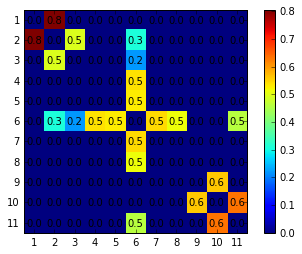
\includegraphics[width=1.3in]{figs/30minmin00conf} & 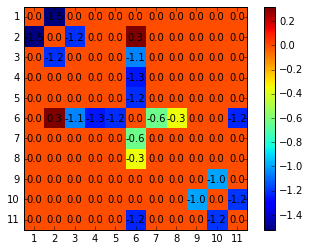
\includegraphics[width=1.3in]{figs/30minmin01conf} & 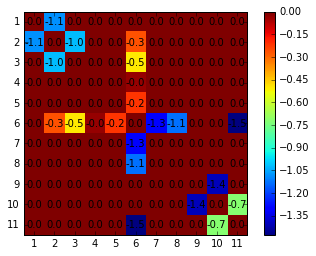
\includegraphics[width=1.3in]{figs/30minmin10conf} & 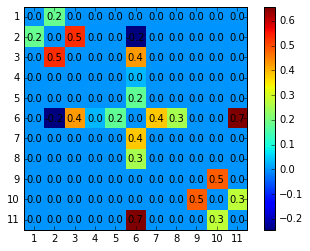
\includegraphics[width=1.3in]{figs/30minmin11conf} \\
(a) (0,0) & (b) (0,1) & (c) (1,0) & (d) (1,1) \\[6pt]
\end{tabular}
\caption{Edge potentials for the IPF run using 30 minute buckets (aggregated using \texttt{min}) in the physically connected Soda AMPlab graph (Figure~\ref{fig:soda_edges}(a)). This model had the \emph{highest} log-likelihood of the IPF run on the physical graph.}
\label{fig:30minminphysical}
\end{figure}

\begin{figure}
\centering
\begin{tabular}{cccc}
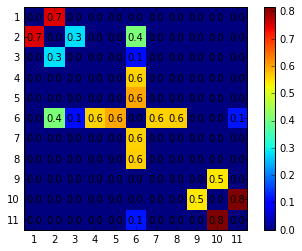
\includegraphics[width=1.3in]{figs/30secmin00conf} & 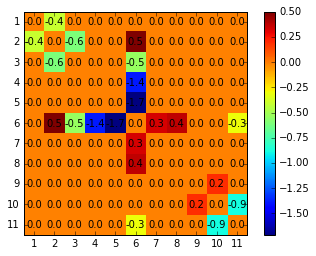
\includegraphics[width=1.3in]{figs/30secmin01conf} & 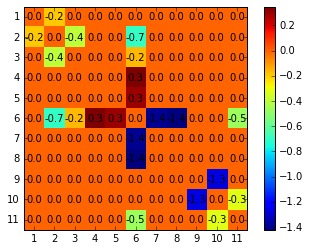
\includegraphics[width=1.3in]{figs/30secmin10conf} & 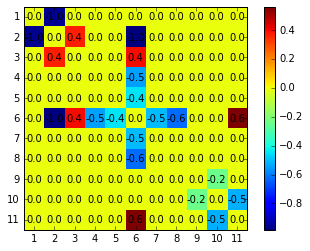
\includegraphics[width=1.3in]{figs/30secmin11conf} \\
(a) (0,0) & (b) (0,1) & (c) (1,0) & (d) (1,1) \\[6pt]
\end{tabular}
\caption{Edge potentials for the IPF run using 30 second buckets (aggregated using \texttt{min}) in the physically connected Soda AMPlab graph (Figure~\ref{fig:soda_edges}(a)). This model had the \emph{lowest} log-likelihood of the IPF run on the physical graph.}
\label{fig:30secminphysical}
\end{figure}

\begin{figure}
\centering
\begin{tabular}{cccc}
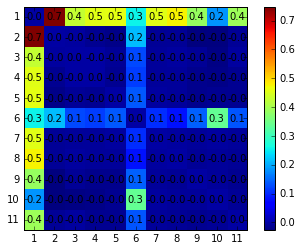
\includegraphics[width=1.3in]{figs/30secmin00fullconf} & 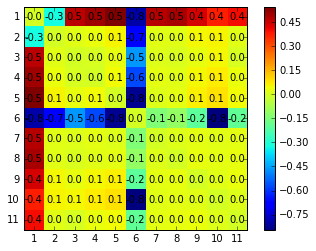
\includegraphics[width=1.3in]{figs/30secmin01fullconf} & 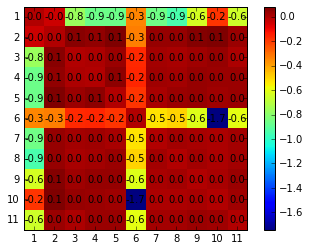
\includegraphics[width=1.3in]{figs/30secmin10fullconf} & 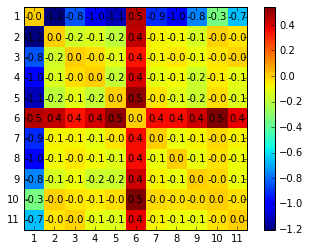
\includegraphics[width=1.3in]{figs/30secmin11fullconf} \\
(a) (0,0) & (b) (0,1) & (c) (1,0) & (d) (1,1) \\[6pt]
\end{tabular}
\caption{Edge potentials for the IPF run using 30 second buckets (aggregated using \texttt{min}) in the fully-connected Soda AMPlab graph (Figure~\ref{fig:soda_edges}(b)). This model had the \emph{lowest} log-likelihood of the IPF run on the fully-connected graph.}
\label{fig:30secminfull}
\end{figure}

\begin{figure}
\centering
\begin{tabular}{cc}
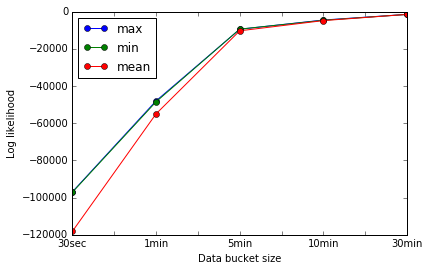
\includegraphics[width=.4\linewidth]{figs/physical_loglikelihood} & 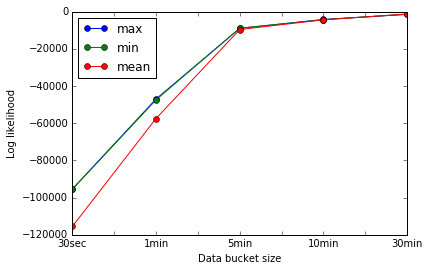
\includegraphics[width=.4\linewidth]{figs/full_loglikelihood} \\
(a) Physical Graph IPF Log Likelihoods & (b) Fully-connected Graph IPF Log Likelihoods \\[6pt]
\end{tabular}
\caption{Plots of the log-likelihood of the IPF runs on the physical and fully-connected graph across different bucket sizes and bucket aggregation functions. We can see that at as the amount of aggregation increases, the log-likelihood increases, and the choice of aggregation function matters less. This is in line with what we would expect, but the converged parameters in the coarser cases may lose some of the subtle interactions between microzones.
It is also interesting to note that the log-likelihoods of the physical and fully-connected graphs are very similar.}
\label{fig:loglikelihood}
\end{figure}

\if 0
Results:
- write it up! visualize
- we plot min/max/mean bucket at diff bucket intervals (30s, 1min 5min 10min 30min):
    - log likelihoods!
- then we interpret the highest log likelihood models:
    - fully connected
    - physically connected
\fi
